\documentclass[master.tex]{subfiles}

\begin{document}

\section*{B. Preliminary}

\subsection*{Prospective memory linking window is longer than retrospective
  linking window for a negative memory}

\begin{wrapfigure}{r}{0.5\textwidth}
  \centering \includegraphics[scale = .4]{Figures/pro_retro_prelim.pdf}
  \caption{\footnotesize Prospective memory linking window is longer than
    retrospective linking window for a negative memory.}
  \label{fig:prelim_pro_retro}
\end{wrapfigure}

In the preliminary study shown in \autoref{fig:prelim_pro_retro}, animals are
put into two distinct contexts separated by various time intervals. In the
``prospective linking'' group, animals received a delayed shock in the first
context, and then explore and get tested in the second context. In the
``retrospective linking'' group, animals explored first context, and then get a
delayed shock in the second context, and then put back to the first context for
testing. Elevated freezing level in the testing context, where no shock ever
occurred for both groups, indicate a transfer of fear and a linking of the two
contexts. For both groups, the exploration and testing session last 10 minutes,
a shock of 0.75 mA was delivered at fifth minute. The various time intervals are
5 hours, 1 day, 2 days and 7 days for both groups.

In prospective linking group, we observed a significant higher freezing level in
testing context with 5 hours interval, but not with either 1 day, 2 days or 7
days interval. This suggest that the fear memories were able to transfer forward
to a neutral context 5 hours in the future. On the other hand, in retrospective
linking group, we observed higher freezing level with either 5 hours, 1 day or 2
days interval, but not with 7 days interval. This suggest the fear memory was
able to transfer backward up to 2 days. Taken together, these results suggest an
extended temporal window of retrospective memory linking comparing to
prospective memory linking.

\subsection*{Negative emotional valence extend temporal window of memory
  linking}

\begin{wrapfigure}{l}{0.5\textwidth}
  \centering 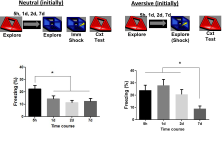
\includegraphics[scale = .4]{Figures/val_retro_prelim.pdf}
  \caption{\footnotesize Negative valence increased temporal window of memory
    linking.}
  \label{fig:prelim_val}
\end{wrapfigure}

In the preliminary study shown in \autoref{fig:prelim_val}, animals are first
put into a neutral context for exploration. After various time interval, animals
are put into a second context. For animals in the aversive group, they received
a delayed shock at fifth minute of the exploration, which associate a negative
emotional value to the second context. For animals in the neutral group, the
exploration of the second context was uninterrupted, and they received a
immediate shock in the second context 2 days after the initial exploration, thus
the emotional valence of the second context was initially neutral for this
group. Both groups were put back to the first context to test for freezing. An
elevated freezing level in the first context indicate a transfer of fear.

For the neutral group, we observed significant higher freezing level in the
first context with 5 hours interval, but not with either 1 day, 2 days or 7 days
interval, suggesting that the two contexts were only linked across 5 hours when
the second context was initially neutral during encoding. On the other hand, we
observed significant higher freezing level with either 5 hours, 1 day or 2 days
interval, but not with 7 days interval, suggesting the two memories were able to
link across 2 days when the second memory was initially negative during
encoding. Taken together, these results suggest that negative emotional valence
was able to extend the time window of memory linking.

\begin{wrapfigure}{r}{0.5\textwidth}
  \centering 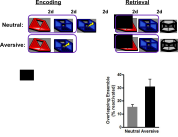
\includegraphics[scale = .4]{Figures/val_retro_prelim_imag.pdf}
  \caption{\footnotesize Negative valence increased the ensemble overlap of two
    memories across 2 days}
  \label{fig:prelim_val_imag}
\end{wrapfigure}

In another preliminary study shown in \autoref{fig:prelim_val_imag}, calcium
imaging was carried out during all the behavior sessions. The experiment design
is similar to the previous behavior study, except the time interval between the
initial exploration of the two contexts was fixed at 2 days, since there was a
significant behavior effect of negative valence at 2 days interval. Consistent
with the behavior results, we found a significant increase in neural overlaps of
the two ensembles during the retrieval of the two contexts in the aversive
group. Interestingly, between the two groups, there is no significant difference
between the neural overlaps of the two ensembles during encoding of the two
contexts, suggesting that the changes in the overlaps of the representation of
the two contexts, possibly memory linking as well, happened during offline
periods between the initial encoding and the testing of the memories.

\subsection*{Minian: a python analysis pipeline for calcium imaging data}

One of the challenge facing miniature microscope in behaving animals is the
analysis of calcium imaging data. Previously, a constrained non--negative matrix
factorization algorithm has been developed to extract calcium traces of
different neurons from raw video. However, a lack of user-friendly interface and
visualization tools for result inspection limit its popularity among community.
Moreover, a method of cross-registering neurons across sessions has not been
integrated into the analysis pipeline. To address these issues and facilitate
the analysis of imaging data, we have developed a pipeline based on jupyter
notebook, which is a document format that combines codes and texts. The adoption
of jupyter notebook enables us to take and share text notes, edit and execute
codes, as well as dynamically visualize results all in an integrated document,
so that we can easily share reproducible analysis to the community
(\autoref{fig:prelim_minian}). Furthermore, a simple cross-registration method
based on euclidean distance of centroids of neurons has been integrated into the
pipeline. Application of this method to our preliminary data shows that the
method could identify same neurons across sessions with satisfactory accuracy.

\begin{figure}[!h]
  \centering \includegraphics[scale = .135]{Figures/minian.png}
  \caption{\footnotesize integration of notes, codes and visualization of
    results in a single document.}
  \label{fig:prelim_minian}
\end{figure}


\end{document}
